%%%%%%%%%%%%%%%%%%%%%%%%%%%%%%%%%%%%%%%%%
% Short Sectioned Assignment
% LaTeX Template
% Version 1.0 (5/5/12)
%
% This template has been downloaded from:
% http://www.LaTeXTemplates.com
%
% Original author:
% Frits Wenneker (http://www.howtotex.com)
%
% License:
% CC BY-NC-SA 3.0 (http://creativecommons.org/licenses/by-nc-sa/3.0/)
%
%%%%%%%%%%%%%%%%%%%%%%%%%%%%%%%%%%%%%%%%%

%----------------------------------------------------------------------------------------
%	PACKAGES AND OTHER DOCUMENT CONFIGURATIONS
%----------------------------------------------------------------------------------------

\documentclass[paper=a4, fontsize=12pt]{scrartcl} % A4 paper and 11pt font size

\usepackage[T1]{fontenc} % Use 8-bit encoding that has 256 glyphs
\usepackage{fourier} % Use the Adobe Utopia font for the document - comment this line to return to the LaTeX default
\usepackage[english]{babel} % English language/hyphenation
\usepackage{amsmath,amsfonts,amsthm} % Math packages

\usepackage{sectsty} % Allows customizing section commands
\allsectionsfont{\centering \normalfont\scshape} % Make all sections centered, the default font and small caps

\usepackage{graphicx}

\usepackage[a4paper,lmargin=2.5 cm,rmargin=2 cm,tmargin=2 cm,bmargin=2 cm]{geometry}

\usepackage{fancyhdr} % Custom headers and footers
\pagestyle{fancyplain} % Makes all pages in the document conform to the custom headers and footers
\fancyhead{} % No page header - if you want one, create it in the same way as the footers below
\fancyfoot[L]{} % Empty left footer
\fancyfoot[C]{} % Empty center footer
\fancyfoot[C]{\thepage} % Page numbering for right footer
\renewcommand{\headrulewidth}{0pt} % Remove header underlines
\renewcommand{\footrulewidth}{0pt} % Remove footer underlines
\setlength{\headheight}{13.6pt} % Customize the height of the header

\usepackage{chngcntr}
%\numberwithin{equation}{section} % Number equations within sections (i.e. 1.1, 1.2, 2.1, 2.2 instead of 1, 2, 3, 4)
%\numberwithin{figure}{section} % Number figures within sections (i.e. 1.1, 1.2, 2.1, 2.2 instead of 1, 2, 3, 4)
%\counterwithout{figure}{section}
%\numberwithin{table}{section} % Number tables within sections (i.e. 1.1, 1.2, 2.1, 2.2 instead of 1, 2, 3, 4)

\setlength\parindent{0pt} % Removes all indentation from paragraphs - comment this line for an assignment with lots of text

\usepackage{amsmath}
\usepackage{float} % To firce the location of figure
\usepackage{subfigure} %For side-by-side figures
\usepackage{lettrine}
%\usepackage{lipsum}
\usepackage{epstopdf} %To read *.eps Files
\usepackage{listings} % To include source codes in LATEX document
\usepackage{mathrsfs} % To include script fonts. use \mathscr{}
\usepackage{courier} % To write in courier fornt
\usepackage{mathtools} % For mat symbols
\usepackage{xfrac} % For \sfrac{}{}
\usepackage{pdfpages} % To insert Pdf files
%----------------------------------------------------------------------------------------
%	TITLE SECTION
%----------------------------------------------------------------------------------------

\newcommand{\horrule}[1]{\rule{\linewidth}{#1}} % Create horizontal rule command with 1 argument of height

\title{	
\normalfont \normalsize 
\textsc{Wright State University\\ Department of Mechanical and Materials Engineering} \\ [25pt] % Your university, school and/or department name(s)
\horrule{0.5pt} \\[0.4cm] % Thin top horizontal rule
\large ME7690 - Vibration Testing and Machine Health Monitoring \\ % The assignment title
\huge Effect of Unbalance Masses on Rotating Machinery\\
\horrule{2pt} \\[0.5cm] % Thick bottom horizontal rule
}

\author{Koorosh Gobal} % Your name

\date{\normalsize\today} % Today's date or a custom date

\begin{document}

\maketitle % Print the title

%----------------------------------------------------------------------------------------
%	SECTION 1
%----------------------------------------------------------------------------------------
\section*{Problem Description}
Rotating machine is one of the most important equipment in industrial applications. Rotating components are used in many engineering applications such as turbo-machinery, internal combustion engines and even computer disk storage. At its most basic level rotating machinery problems are concerned with one or more mechanical structures (rotors) supported by bearings and influenced by internal phenomena that rotate around a single axis. More than often, the rotor experience unbalances due to the manufacturing defects. Unbalance is caused when the center of mass is out of alignment with the center of rotation. When rotating, this can cause unwanted vibration that can cause a reduction in the life of the components. In this experiment the rotating machinery setup is used to model the rotating unbalance and its effect on the support bearings. \emph{Kurtosis} and \emph{ensemble averaging} are used in this lab for processing the results.
%----------------------------------------------------------------------------------------
%	SECTION 2
%----------------------------------------------------------------------------------------
\section*{Experimental Setup}
The expertimanetal setup is shown in Figure ~\ref{fig:experimentalSetup}. Three separate stud accelerometers are used to gather the data. These are shown in Figure ~\ref{fig:experimentalSetup} using red arrows. These record the vibrating response of the motor and each of the bearings. In order track the rotation of shaft, an optical transducer is used in this setup. The optical transducer is shown with blue arrow in Figure ~\ref{fig:experimentalSetup}. A notch is cut on the beam as a reference for the optical transducer to follow. This is reflected as spikes on the voltage output of optical transducer.\\

For the data acquisition, the motor is run at $40$Hz. The sampling period is chosen as $1.2798$ seconds. The bandwidth is also selected as $5000$Hz. The data acquisition is triggered after the transient effects has been damped out. We look the transient time roughly as $60$ seconds. Two seprate experiments were done using this setup. For the first experiment, the system was run without any additional eccentric mass. On the second setup, an eccentric mass was applied at the disc using bolts and the experiment was repeated to gather the data. These two data sets are compared in the following sections.
%
\begin{figure}[H]
	\centering
	\includegraphics[height = 8.5cm]{setup.jpg}
	\caption{The experimental setup.}
	\label{fig:experimentalSetup}
\end{figure}
%
%----------------------------------------------------------------------------------------
%	SECTION 3
%----------------------------------------------------------------------------------------
\section*{Results and Discussion}
The first step in processing the results is to break the output data into ensembles. This can be done using the data from the optical transducers. In this regard, instances where the voltage spikes in the ODT output data occurred were recorded and used for breaking the data from accelerometers into ensembles. It is worthwhile to mention that the motor frequency picked by the ODT was $39.6285$ which is really close to the frequency of the motor shown on the control board. The averaged ensemble data and the actual signal in each rotation is shown in Figure ~\ref{fig:result}. It is clear that ensemble averaging will remove the noise from the signal considerably.
%
\begin{figure}[H]
	\centering
%	\subfigure[Motor mounted accelerometer]
%	{
%		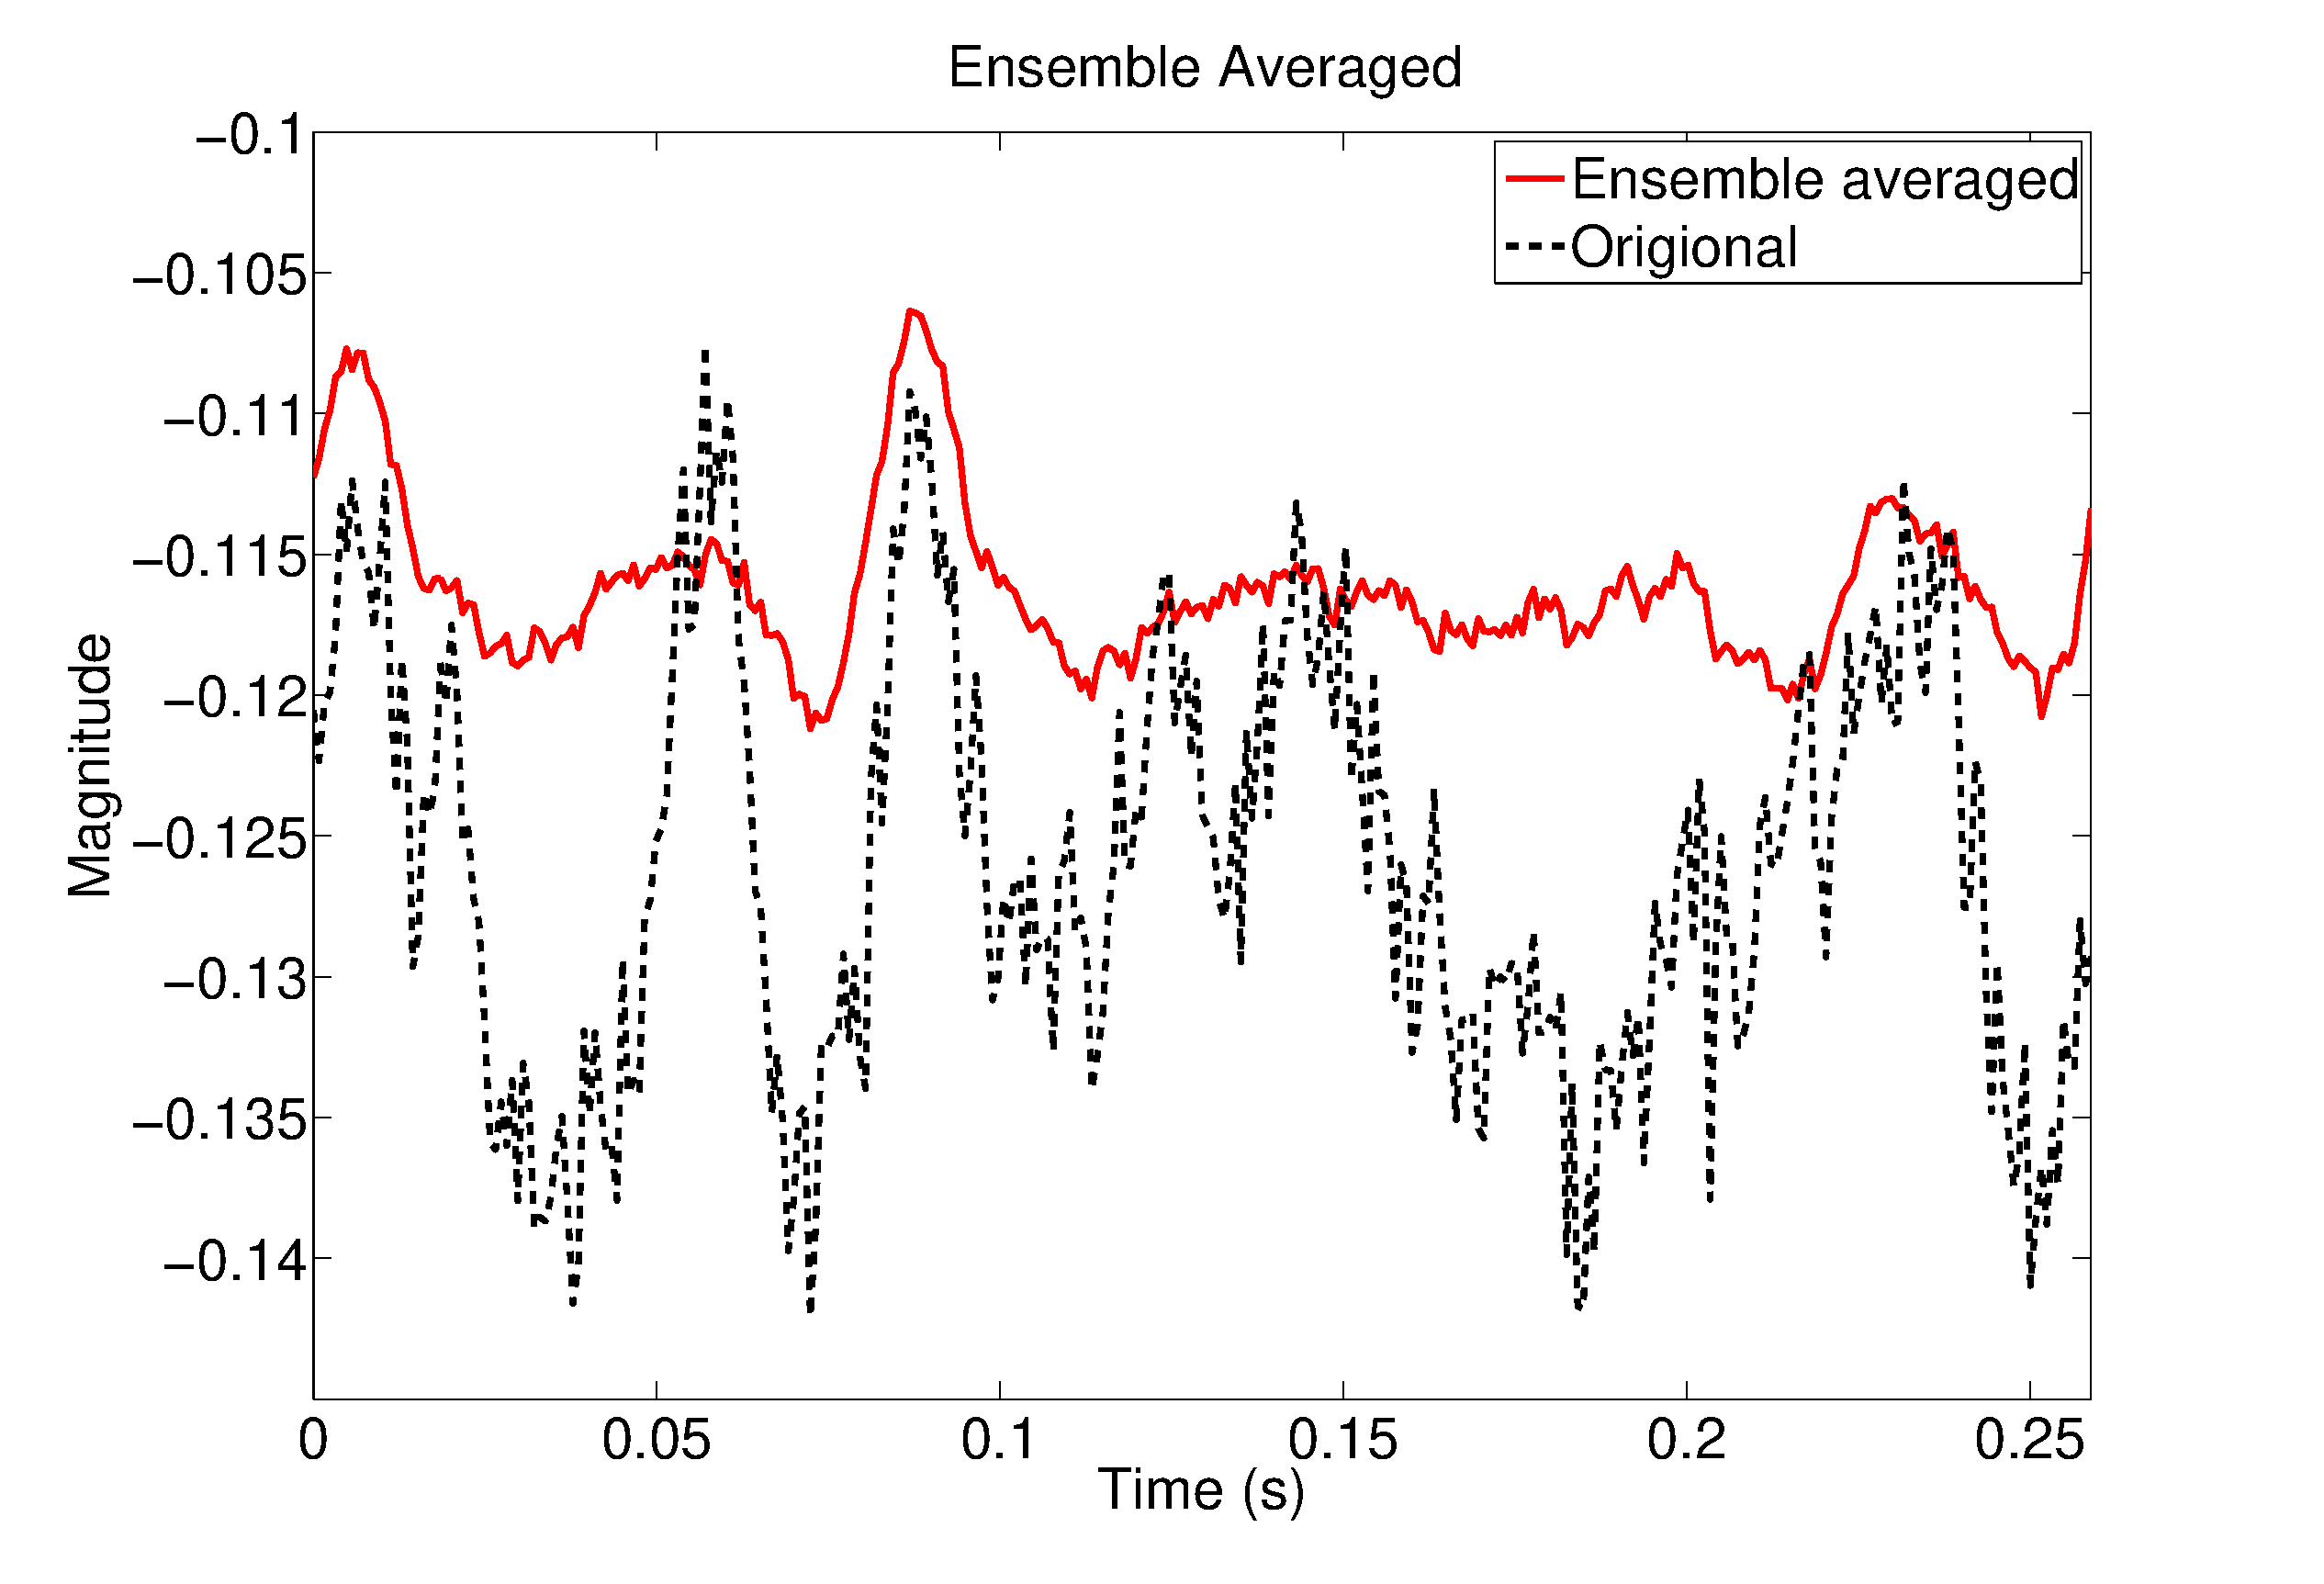
\includegraphics[height=7.0cm]{1_ensembleAve.eps}
%		\label{fig:experimentalSetup1}
%	}
%	\\
	\subfigure[Left bearing accelerometer]
	{
		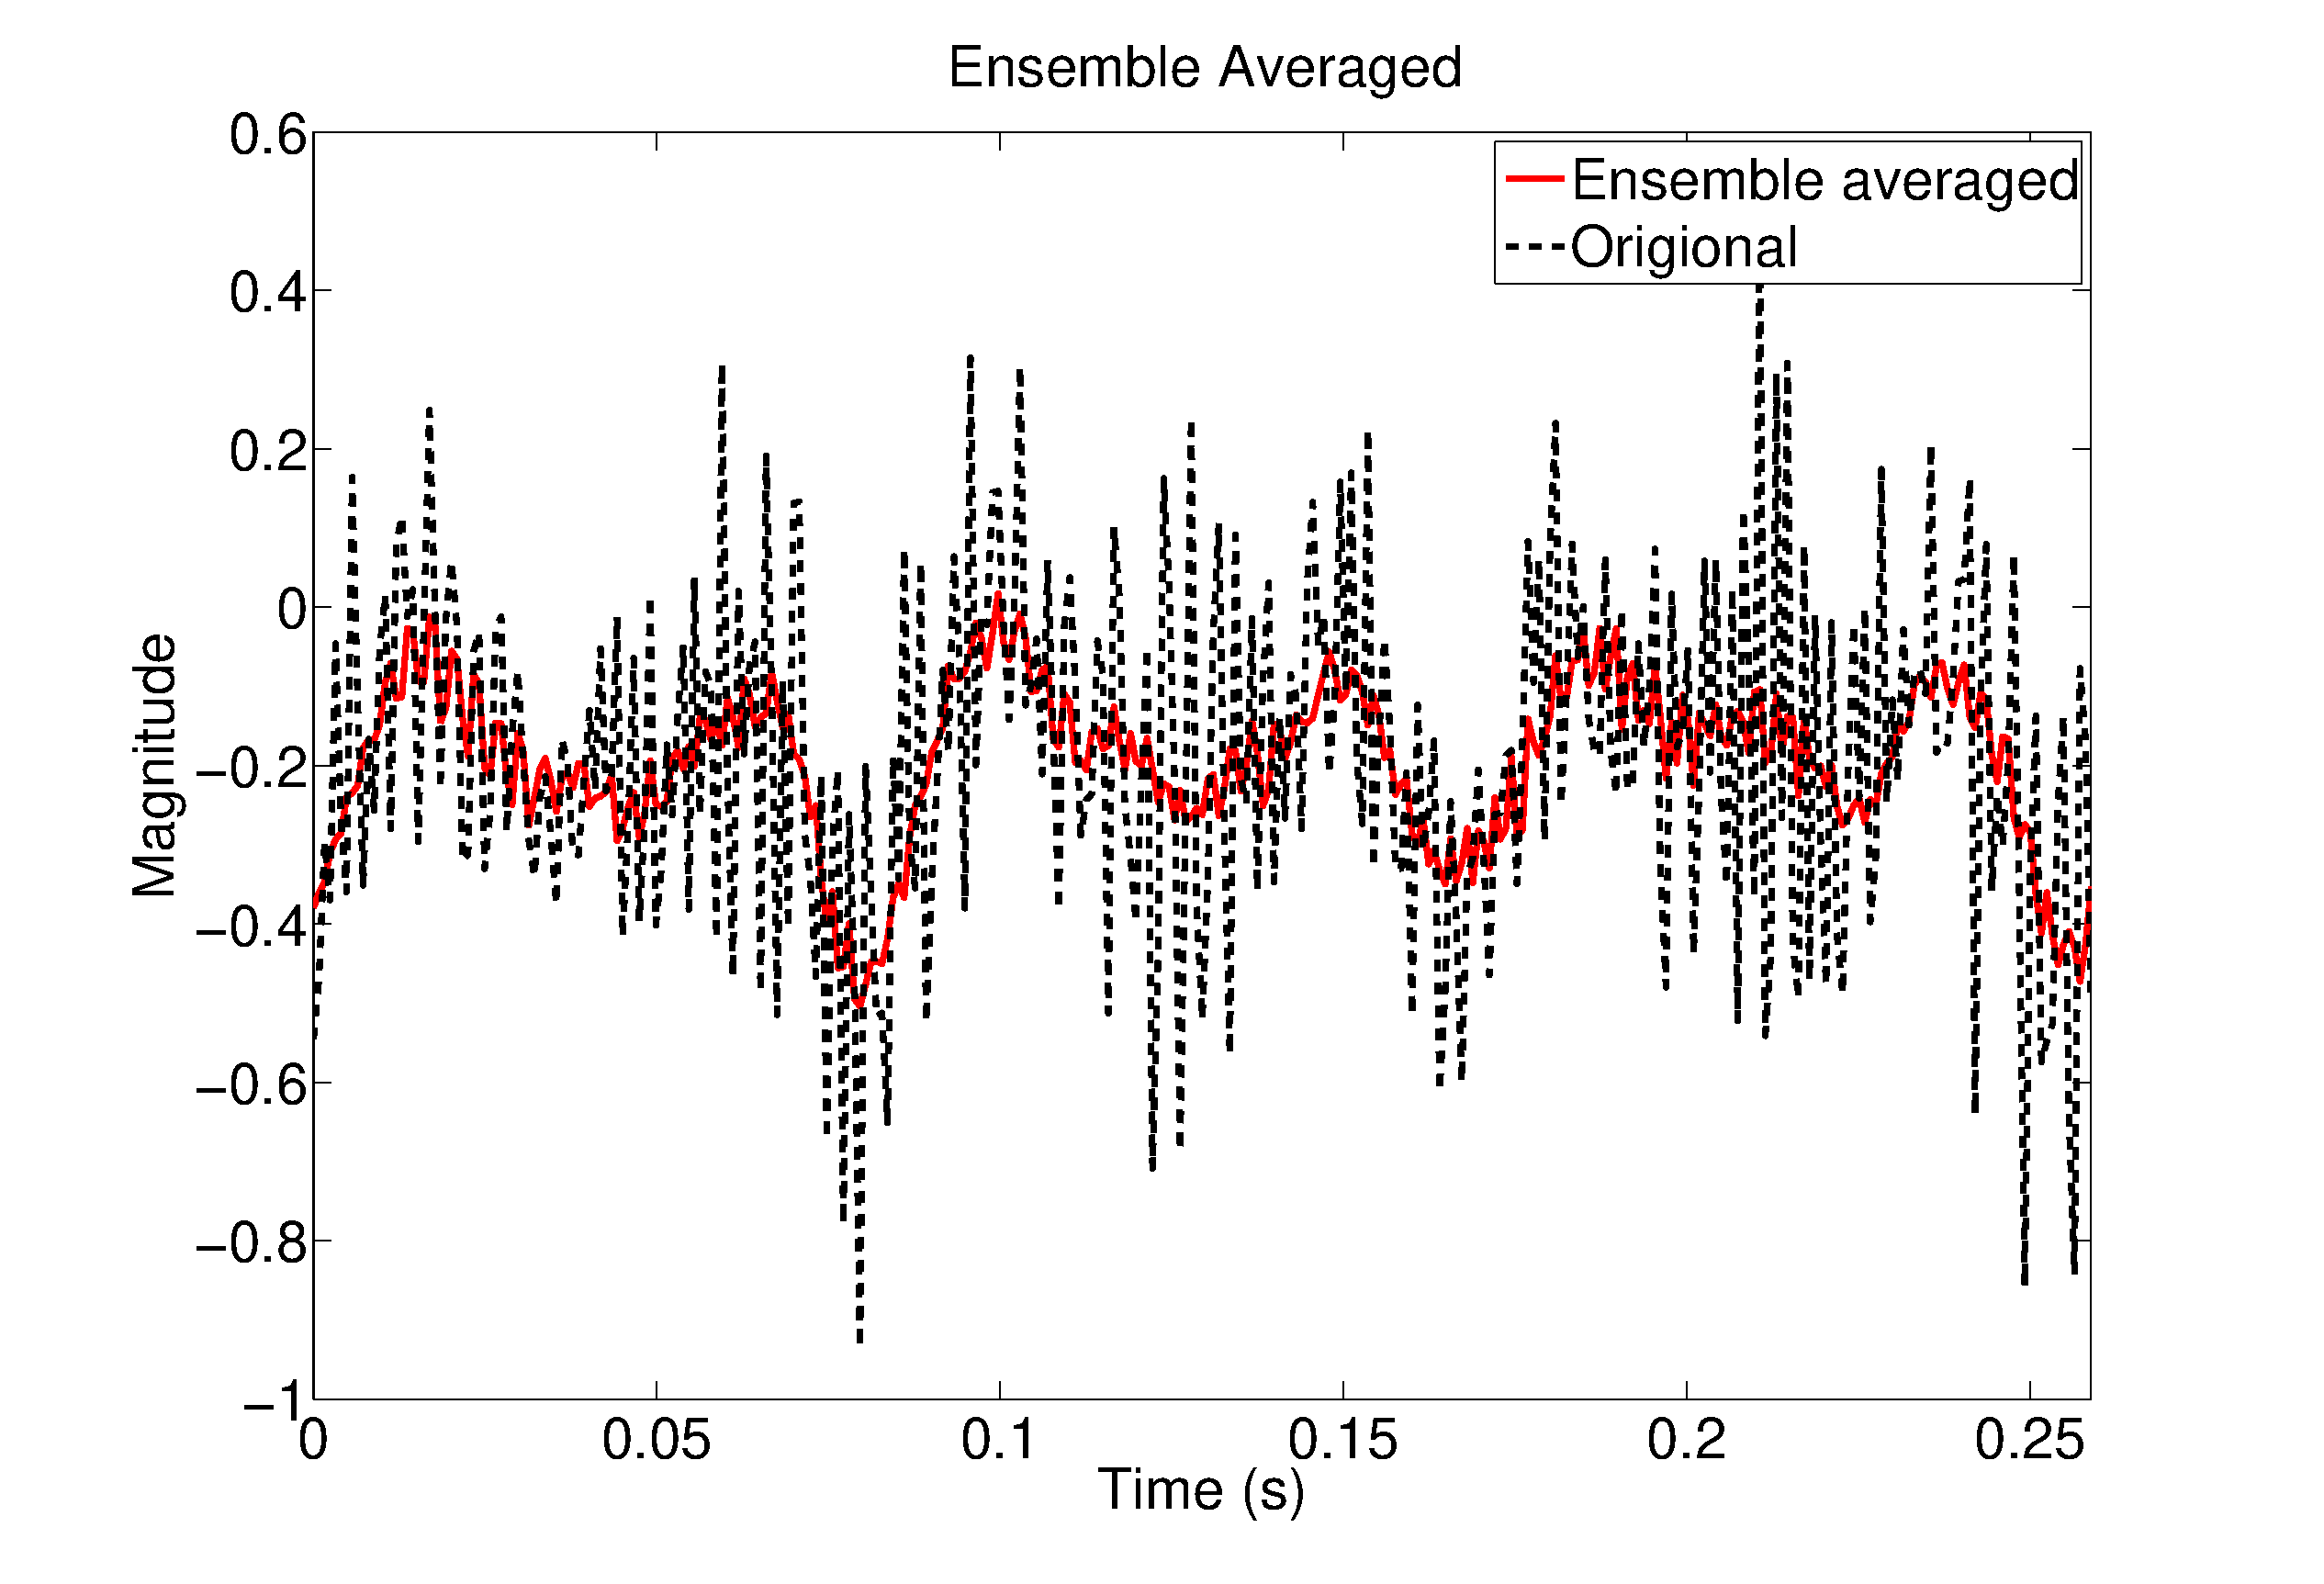
\includegraphics[height=7.0cm]{2_ensembleAve.eps}
		\label{fig:experimentalSetup2}
	}
	\\
	\subfigure[Right bearing]
	{
		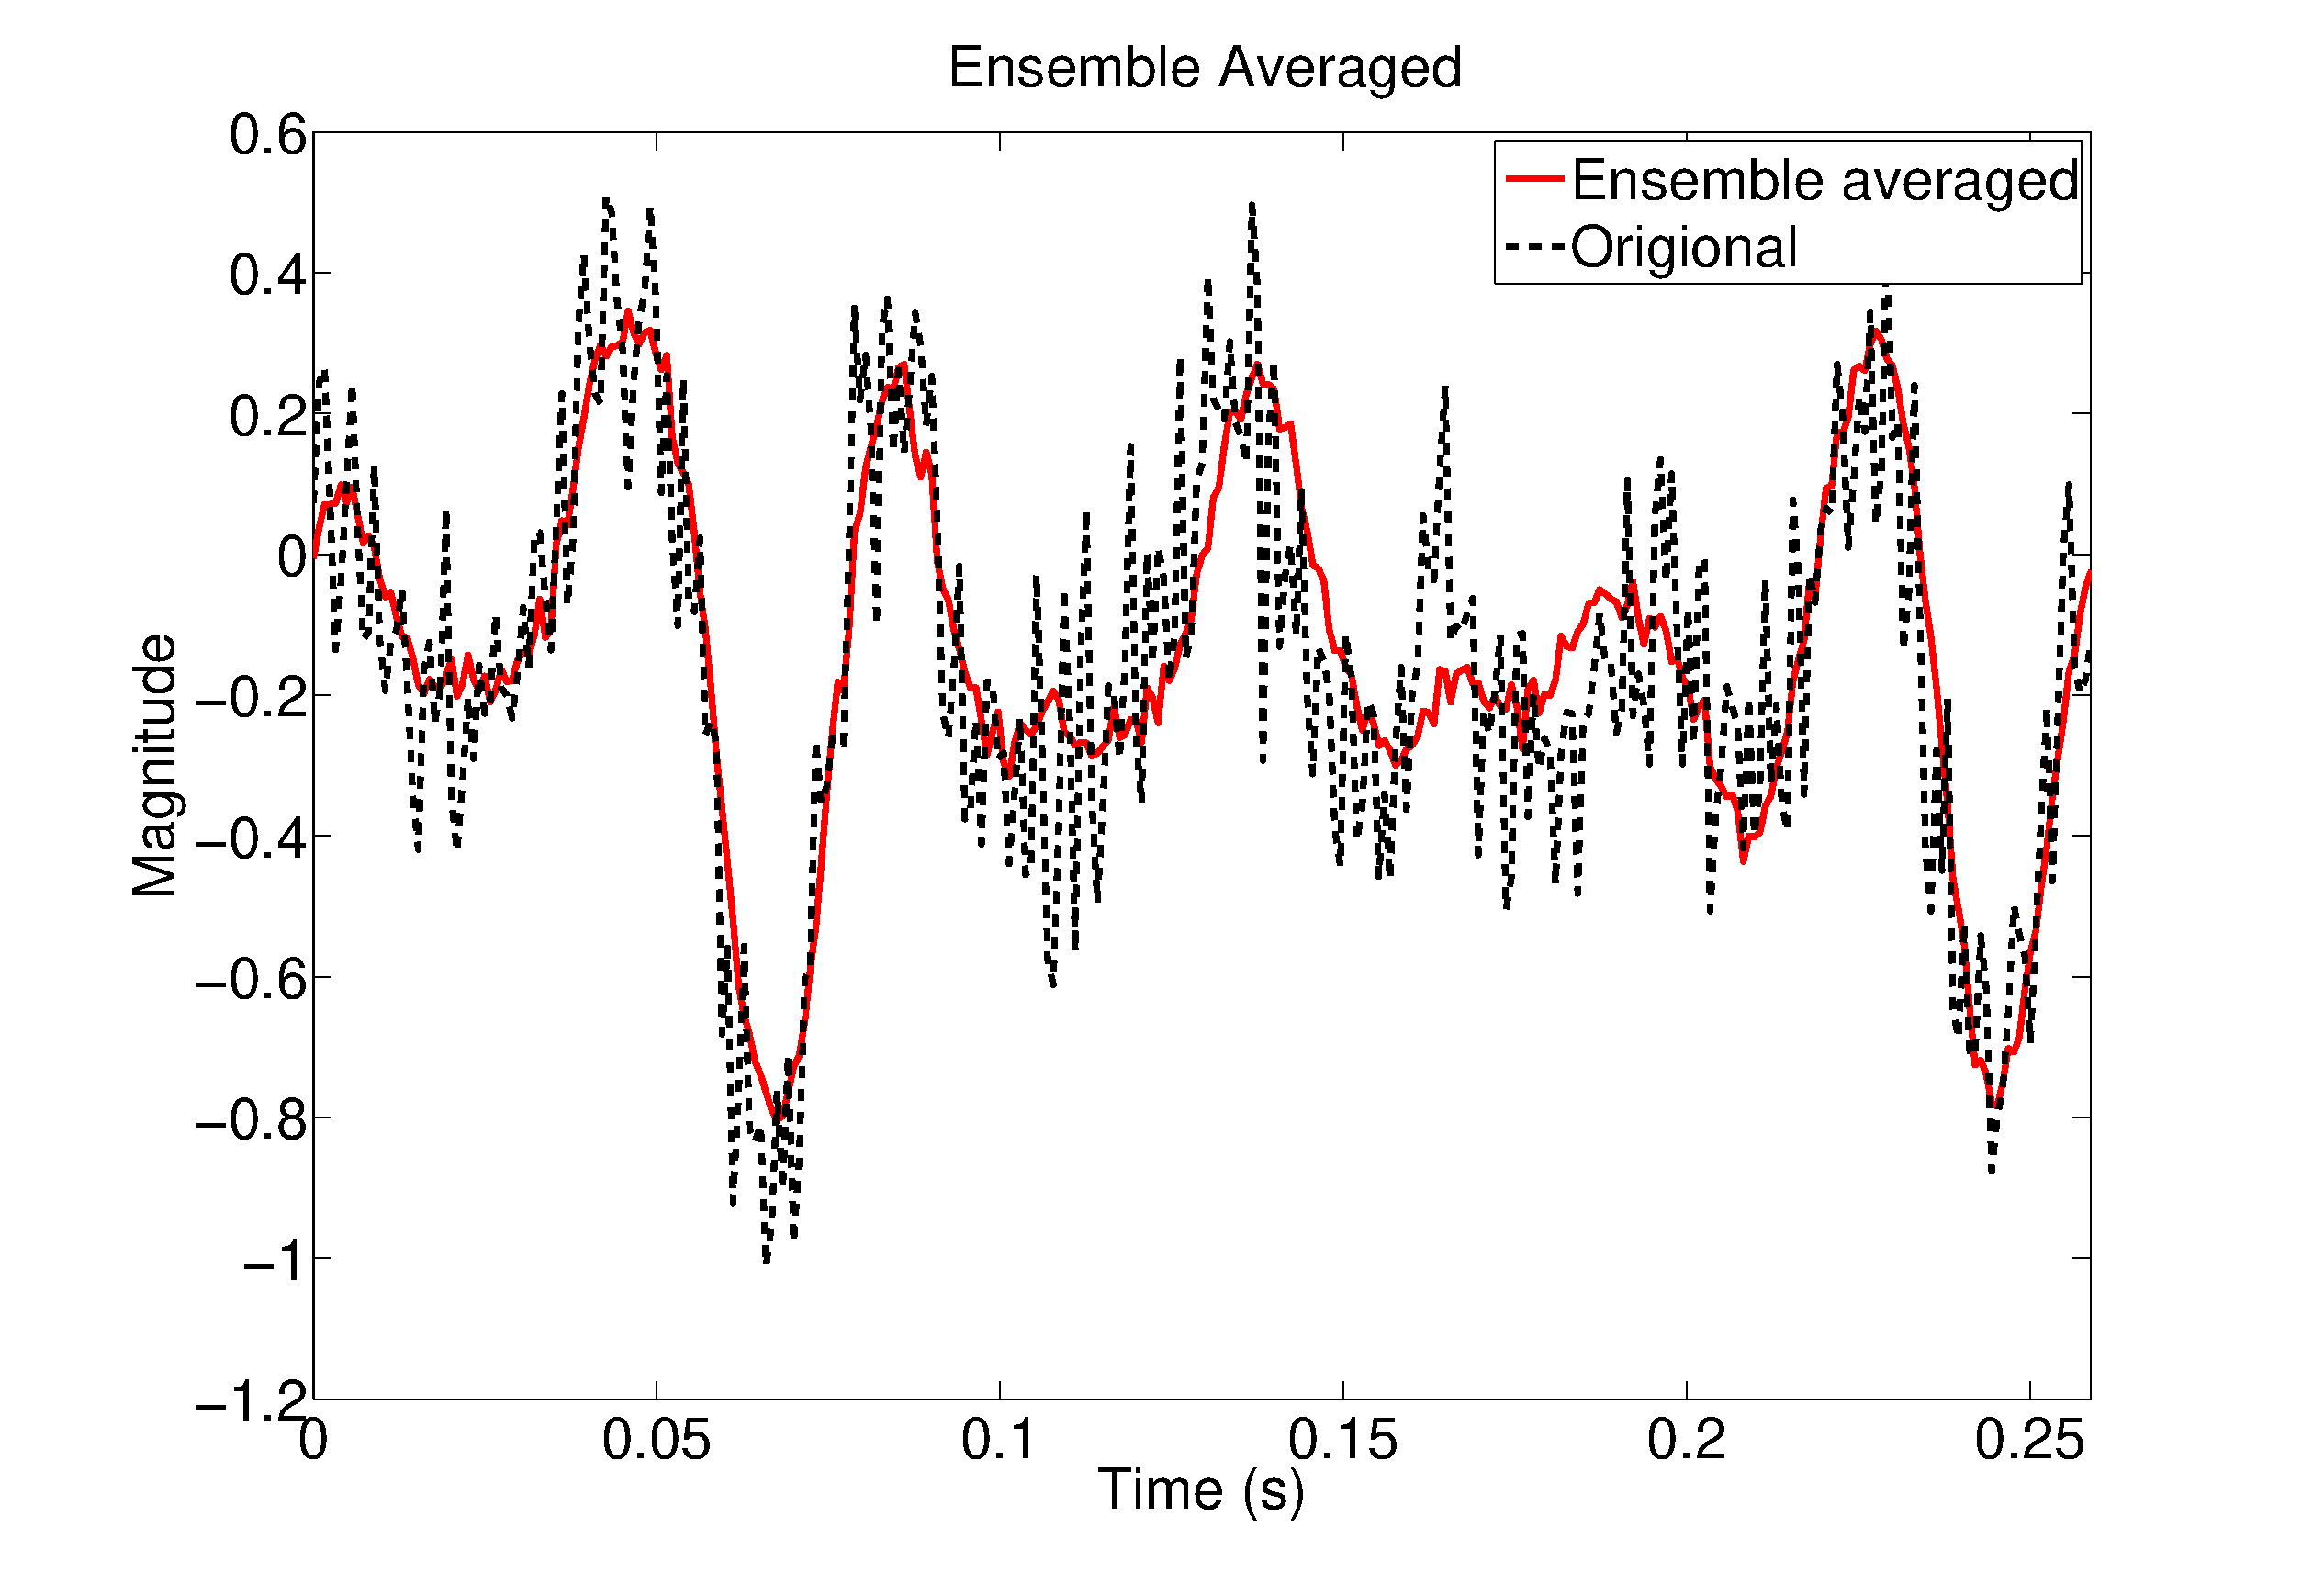
\includegraphics[height=7.0cm]{3_ensembleAve.eps}
		\label{fig:experimentalSetup2}
	}
	\caption{Comparison between the ensemble averaged and original data in single period for a disk \underline{without} rotating unbalance.}
	\label{fig:result}
\end{figure}
%
Another set of data for a case with unbalance mass is gathered is and compared with the original data. The unbalance mass was placed approximately on the angular position of $180$ degree. The zero of the position is selected as the position of the notch. Therefore, it is expected to see a spike on the accelerometer data in the middle of the period of the data. The results for the \lq\lq unbalanced mass \rq\rq\ is also averaged over the ensembles to remove the noise. The results are shown in Figure ~\ref{fig:unbalanceMassTimeDomain}. As is shown in Figure ~\ref{fig:unbalanceMassTimeDomain} the spikes are happening at the half of the period is the time domain data.
%
\begin{figure}[H]
	\centering
	\subfigure[Left bearing]
	{
		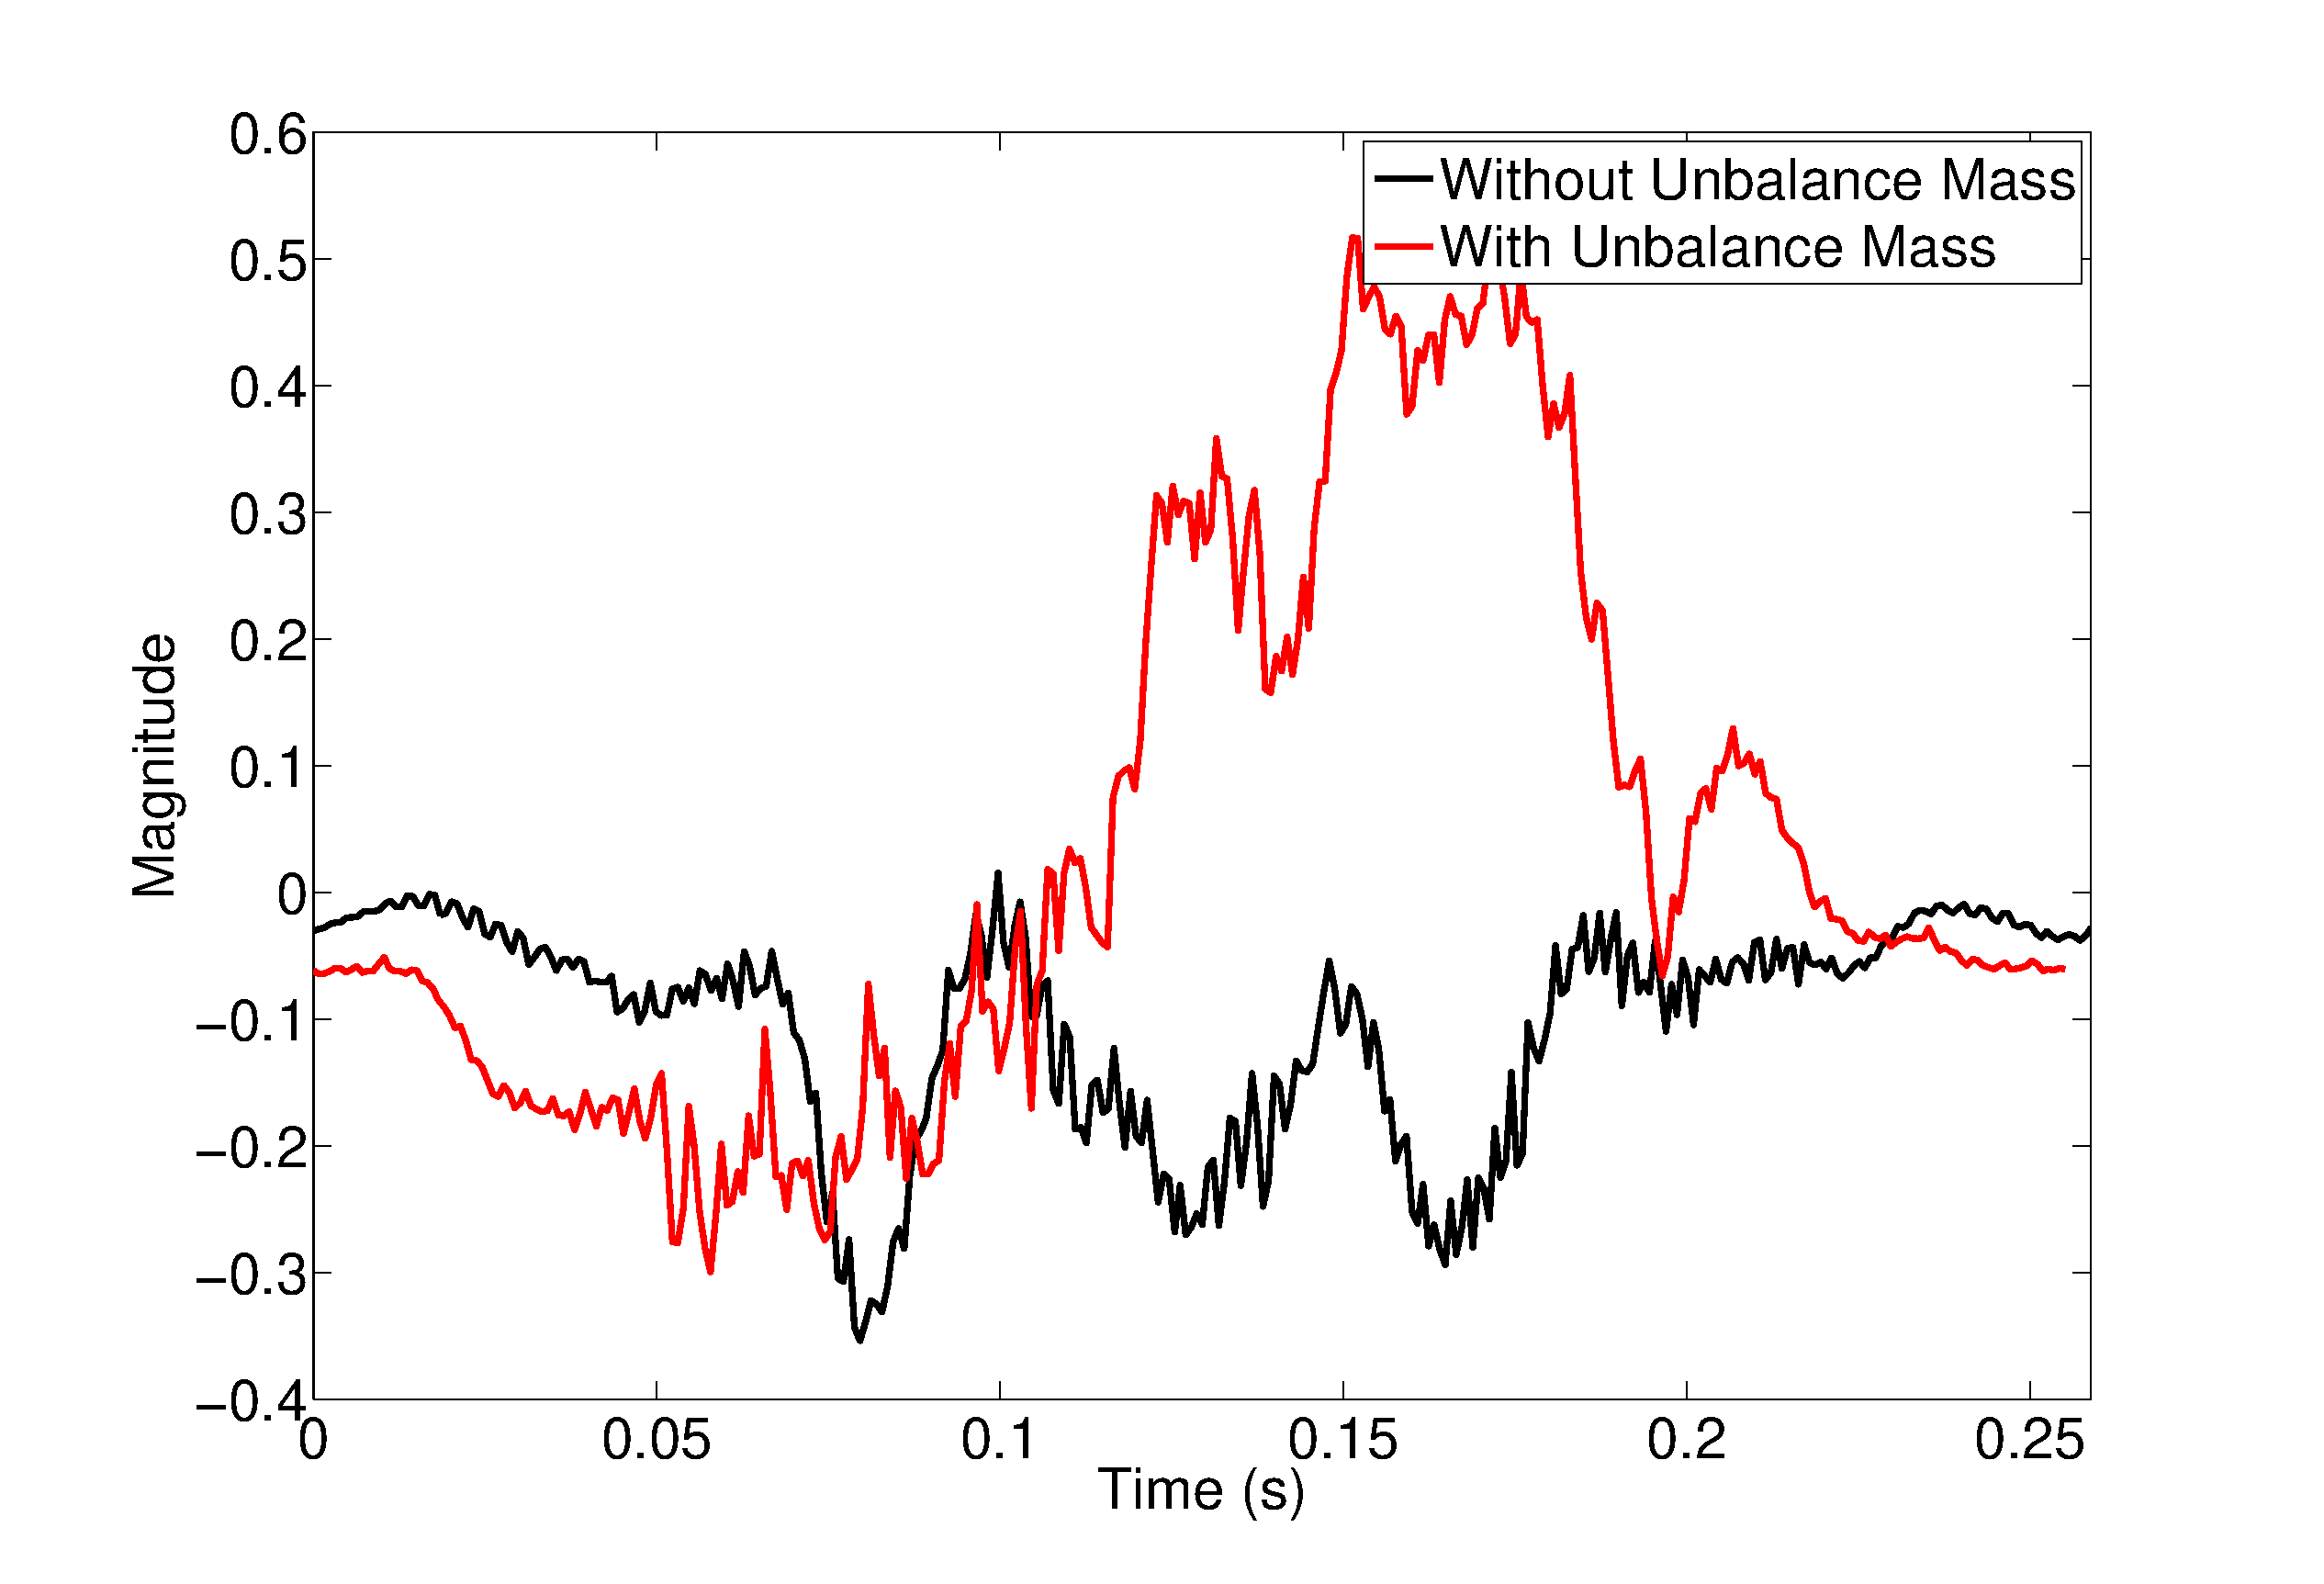
\includegraphics[height=7.0cm]{time_left.eps}
		\label{fig:experimentalSetup1}
	}
	\\
	\subfigure[Right bearing]
	{
		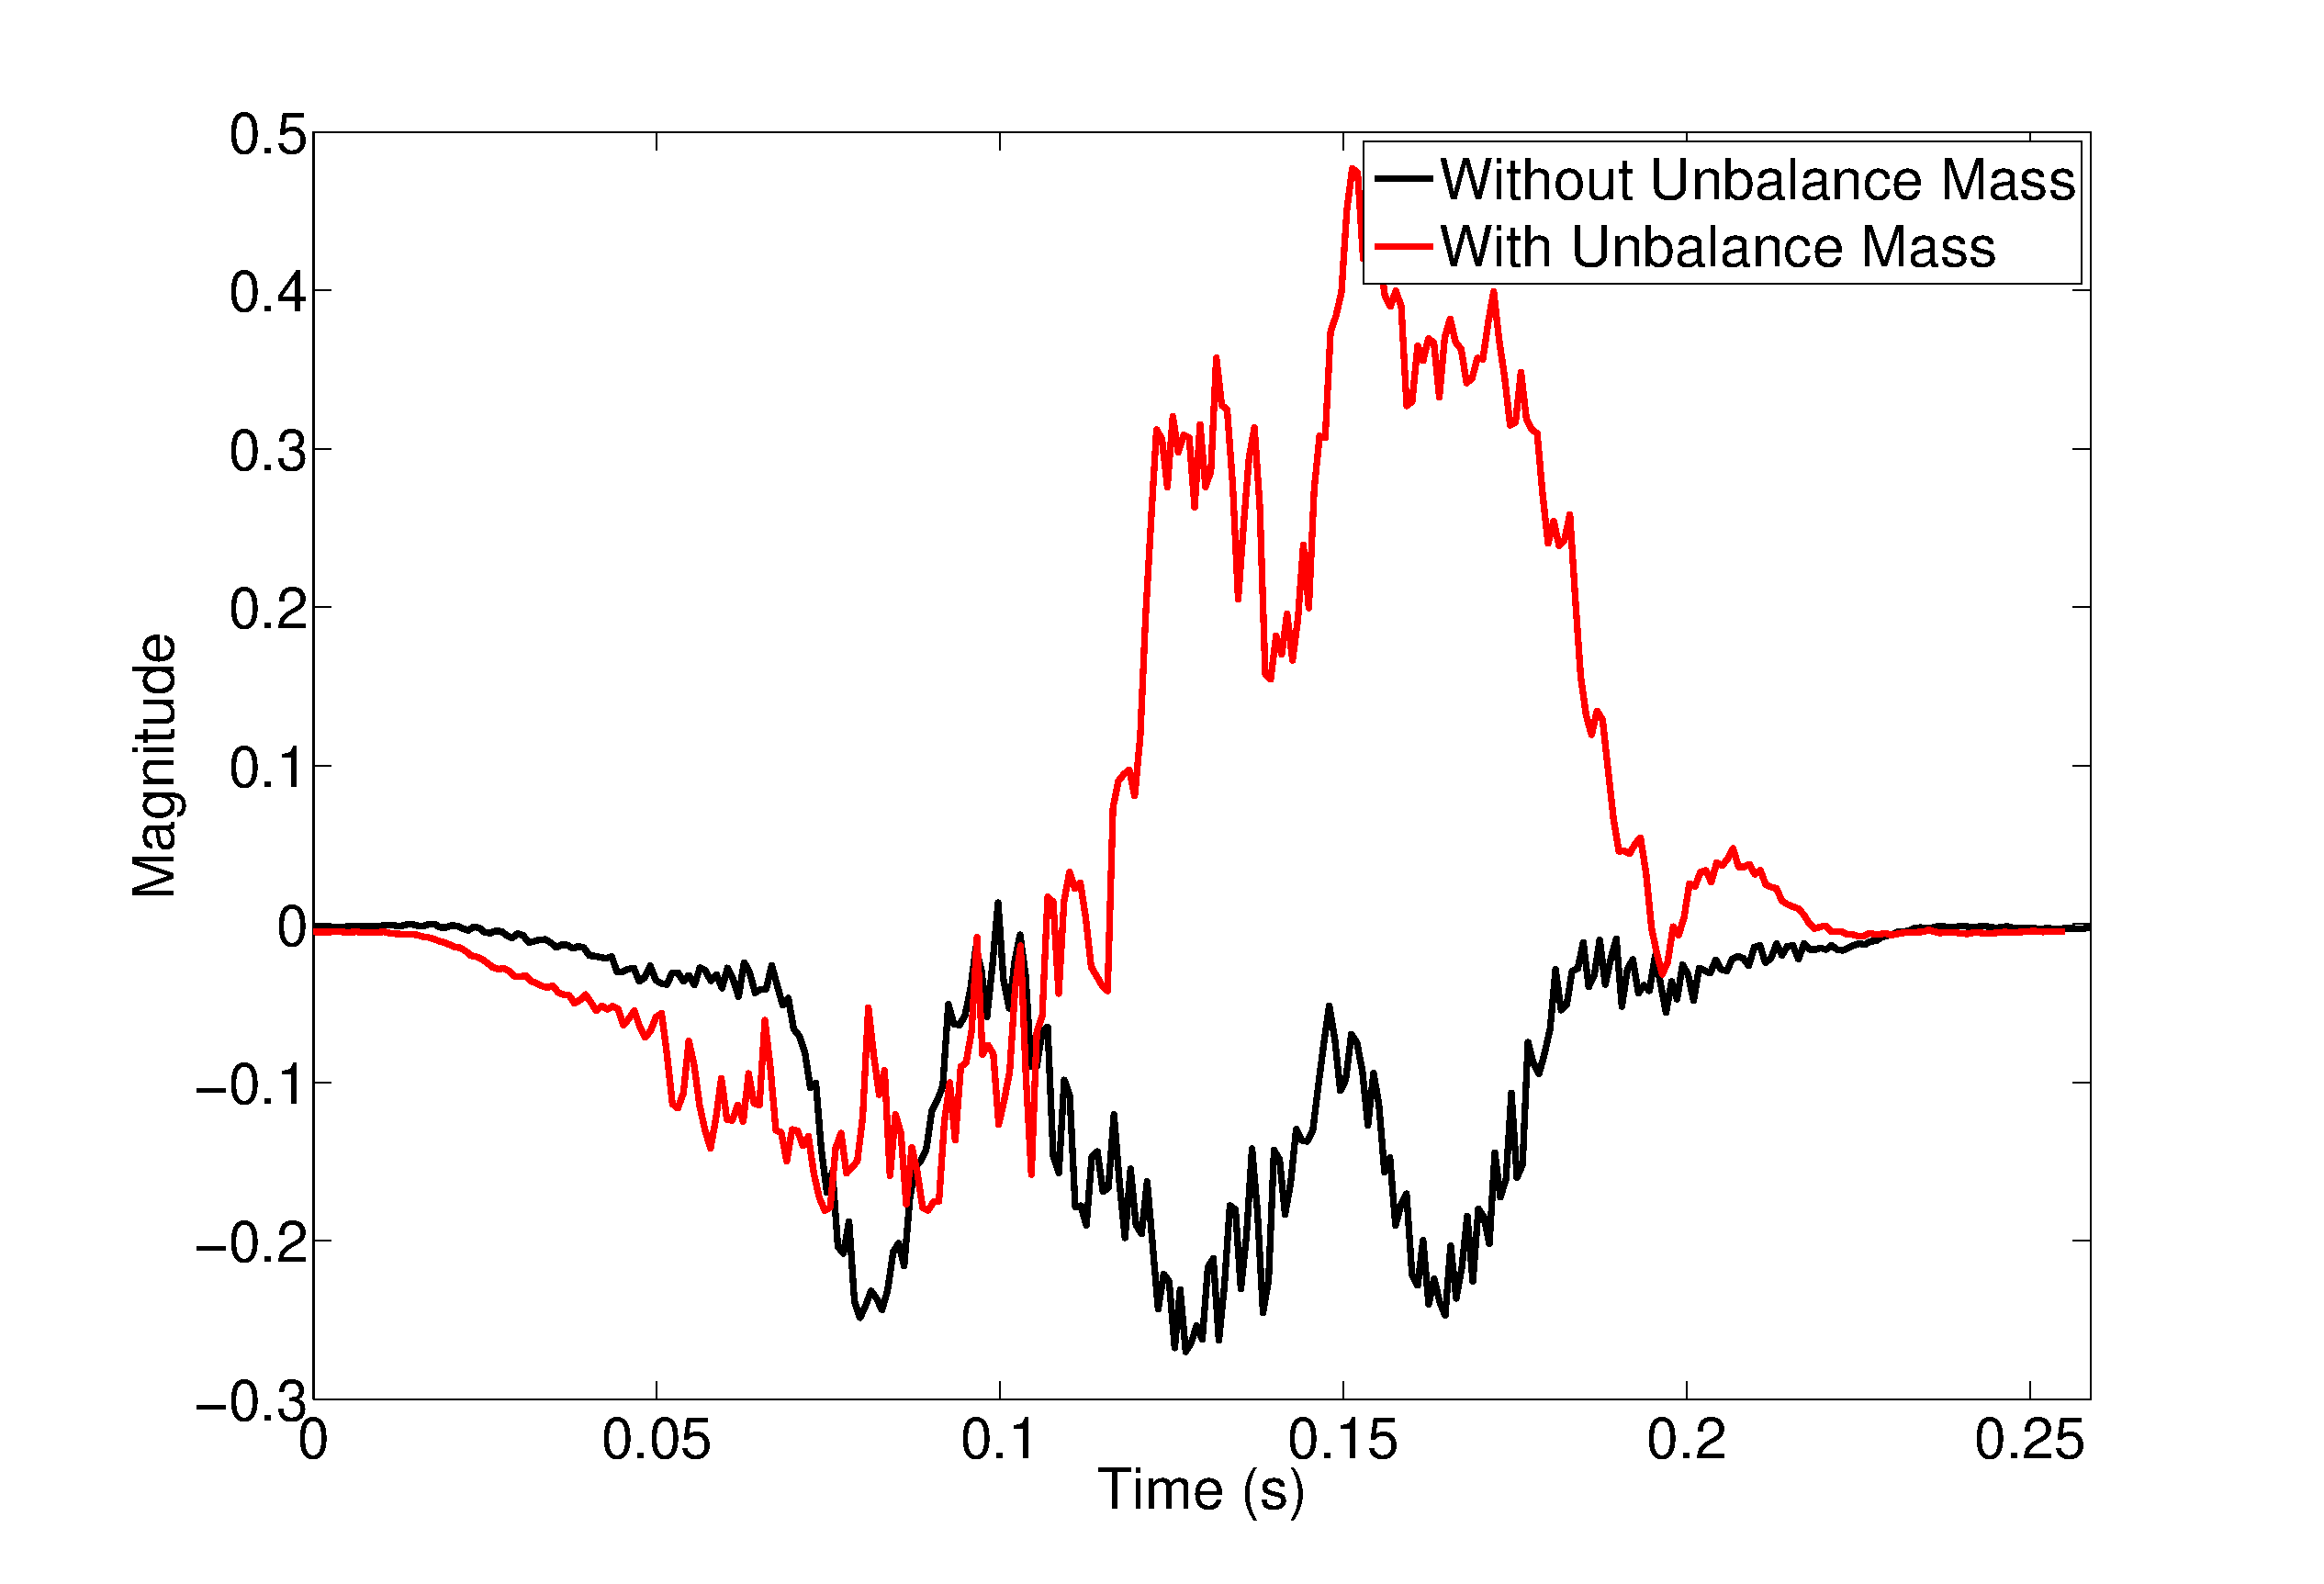
\includegraphics[height=7.0cm]{time_right.eps}
		\label{fig:experimentalSetup2}
	}
	\caption{Effect of unbalance mass on the forces applied on bearings.}
	\label{fig:unbalanceMassTimeDomain}
\end{figure}
%
After averaging the ensembles to remove the noise, the faults in the bearings of the system can be detected by studying the \emph{kurtosis} of the system. It has been demonstrated that spectral kurtosis has a potential for detecting and characterizing transient signals buried in additive noise \cite{antoni2006spectral}. Spectral kurtosis ideally takes zero values at those frequencies where stationary Gaussian noise only is present and high values at those frequencies where transients occur. Figure ~\ref{fig:kurtosis_example} illustrates a signal captured on a faulty rolling element bearing.\\

Given that the nominal kurtosis value of a Gaussian distribution is $3$, the \emph{bias-adjusted kurtosis} value is often used instead. The bias-adjusted kurtosis value is simply calculated by subtracting $3$ from the original value of the kurtosis. Thus for a system with no shock response has a bias-adjusted kurtosis value of $0$. A response near resonance will thus typically cause a bias-adjusted kurtosis value of between $-1.5$ and $0$ \cite{Slater2002vibration}. The bias-adjusted kurtosis for both cases is shown in Table ~\ref{table:results}. The kurtosis is calculated using Matlab's function \texttt{kurtosis} for ensemble averaged data. The near zero value for the bias-adjusted kurtosis of first case demonstrate the the system bearings are healthy. The negative values for the bias-adjusted kurtosis of unbalance system, demonstrates that the system is working near its resonance frequency.
%
\begin{figure}[H]
	\centering
	\includegraphics[height = 7.0cm]{kurtosis_example.jpg}
	\caption{(a) A typical vibration signal measured on a system with a faulty rolling element bearing (inner race fault). Note the high kurtosis value. (b) The same vibration signal in the case of a weak ball fault masked by surrounding noise: the kurtosis is almost zero \cite{antoni2006spectral}.}
	\label{fig:kurtosis_example}
\end{figure}
%
%
\begin{table}[H]
\centering
\begin{tabular}{ c | c | c }
		Case & Left Bearing & Right Bearing \\
	\hline                       
	\hline
		without unbalance mass & 0.40611 & 0.19478 \\
		with unbalance mass & -1.167 & -0.96103 \\
	\hline  
\end{tabular}
\caption{Kurtosis results.}
\label{table:results}
\end{table}
%
%----------------------------------------------------------------------------------------
%	END
%----------------------------------------------------------------------------------------
\bibliographystyle{aiaa}  
\bibliography{ref}
\end{document}